\subsection{Case Study: Service Mesh and Microservice}
\label{s:case-mesh}

Service mesh is a representative pattern which injects a \emph{sidecar} container (proxy) into each microservice Pod, leading to both resource and communication latency challenges.
We illustrate how \sys can utilize \os to optimize the costs caused by proxy-related infra-containers.

% \subsubsection{Service Mesh Background}
\myparagraph{Baseline systems with Istio.}
Besides the basic proxy design (Fig.\ref{fig:intro-wingman}-a),
Istio~\cite{istio} (SOTA mesh system) supports an advanced architecture, \emph{waypoint} sidecar~\cite{istio-ambient} (Fig.\ref{fig:intro-wingman}-b), that can effectively mitigate costs.
Specifically, it decouples the sidecar into a \emph{zero-trusted tunnel} (ztunnel) and a \emph{waypoint sidecar}.
Ztunnel can be shared by all apps on a node for L4 policies, while a waypoint sidecar is dedicated to an app (for L7 policies) and can be scheduled to other nodes.
The decoupling can save resources on the apps' node, however, it also increases the latency for the normal path resulting from the scheduling of waypoint sidecars on a third server.


\myparagraph{\mesh.}
We design \mesh to balance performance and scalability with efficient offloading of sidecars to DPUs with \os.
\mesh supports two deployment methods:
(1) offloading all proxy-related infra-containers (ztunnel and waypoint) to DPU (Fig.\ref{fig:intro-wingman}-d), so that CPU can focus on running microservice apps,
and (2) offloading waypoint containers to DPU (Fig.\ref{fig:intro-wingman}-c).
It will launch new ztunnel and waypoint containers to CPU when DPU devices fail or their resources are insufficient to ensure the availability and QoS of microservices.
If the client and server microservices are on the same node, \mesh will deploy the ztunnel and waypoint containers in the CPU when possible.
\mesh will utilize \giptable to support indrect communication between apps and proxy, and rely on \gsocket to speed up the communication latency.

\myparagraph{Methodology.}
We deploy DeathStarBench~\cite{10.1145/3297858.3304013} and FunctionBench~\cite{kim2019practical} as microservices, and deploy each microservice with an Istio waypoint (using Envoy) as gateway to evaluate the performance of \mesh.
All incoming and outgoing traffic of microservices will be intercepted and processed by the ztunnel on the node.
% where the microservice is located.
We compare \mesh with two systems: IstioCPU and IstioBaselineDPU.
IstioCPU will only deploy microservice Pods on the CPU, which represents the best performance in many cases, but can not effectively utilize DPUs to improve the scalability.
IstioBaselineDPU is implemented based on Istio to deploy microservice Pods on both CPU and DPU (priorly scheduled to DPU).
It represents existing approaches utilizing DPU using pod granularity.
%\mesh-Strawman represents existing approaches to deploy both microservices on CPU and DPU using Pod granularity, which can achieve better scalability.

% \subsubsection{End-to-End Performance}
\myparagraph{End-to-end performance.}
% We evaluate the end-to-end latency of microservices under two baseline systems, \sys-WP (Fig.~\ref{fig:intro-wingman}-c) and \sys-All (Fig.~\ref{fig:intro-wingman}-d).
% To illustrate the benefits of \emph{dynamic split}, \mesh does not use \gsocket in this case.
We evaluate microservices' end-to-end latency under two baseline systems, \sys-WP (Fig.~\ref{fig:intro-wingman}-c) and \sys-All (Fig.~\ref{fig:intro-wingman}-d). 
To show \emph{dynamic split}'s benefits, \mesh does not use \gsocket here.
% All cases use the kernel network stack for network communication.
%We use both FunctionBench and Deathstar in this case.

The evaluation results for FunctionBench are shown in Fig.\ref{fig:eval-mesh-big}-a.
%The test results show that
% Compared with the IstioBaselineDPU, \mesh can shorten microservices' end-to-end latency by 50\%--60\% (dd, pyaes, chameleon), 34\% (gzip-compression), 17\% (video-processing, linpack), and 6\%--7\% (matmul, cnn-image-classification). 
Compared with the IstioBaselineDPU, \mesh can shorten microservices' end-to-end latency up to 60\% (dd, pyaes, chameleon). 
The performance of all apps is improved after deploying with \mesh.
Compared to only using CPU, using \mesh-WP to offload waypoint to DPU only brings end-to-end latency overhead of less than 5\%.
Using \mesh-All to offload ztunnel and waypoint to DPU can saves more CPU resources, and only brings end-to-end overhead of 1\%-2\%(dd, pyaes)  and $<$1\% for all other apps.
%(matmul, gzip-compression, chameleon, cnn image classification, video-processing) and .
%The reason why the end-to-end latency overhead of using \mesh-All is smaller than that of \mesh-WP is perhaps that after the service mesh infrastructure is fully offloaded to DPU, the microservices running on the CPU are subject to less competition for CPU resources and microarchitecture resources (such as cache and TLB), which helps to shorten the running time of microservices.
The reason why the end-to-end latency overhead of using \mesh-All is smaller than that of \mesh-WP is that after the service mesh infrastructure is fully offloaded to DPU, the microservices running on the CPU are subject to less competition for CPU and microarchitecture resources (such as cache and TLB), which helps to shorten the running time of microservices.
The evaluation results for DeathStar are shown in Fig.~\ref{fig:eval-mesh-big}-b.
We do not offload ztunnel here as microservices in DeathStar have short runtime latency.
%As we can see,
\mesh can achieve 29\%--74\% better latency compared with BaselineDPU, and it incurs only $<$1.2ms latency costs (on average) compared with CPU (the ideal performance without offloading).

\myparagraph{Scalability.}
%We compare the scalability of the \mesh and IstioBaselineDPU under high density.
We compare the scalability under high density.
Specifically, both \mesh and IstioBaselineDPU will use all DPU and most CPU resources to deploy Pods.
Each microservice pod is paired with a waypoint proxy.
The total number of microservices and waypoints is the same (70 instances), and the same resources (CPU and memory) are allocated, i.e., 128MB memory and 100 mCPU per waypoint, and 256MB memory and 300 mCPU per app.
We use Pyaes as the testcase.
Requests are evenly load-balanced to all microservices in a random manner using Nginx.

The average latency results are presented in Fig.\ref{fig:eval-mesh-big}-c/d and the P99 latency in Fig.\ref{fig:eval-mesh-big}-e/f.
%The results show that 
Under different RPS, microservices deployed using \mesh achieve better performance than the IstioBaselineDPU --- 39\% improved end-to-end latency.
When the RPS rises, the latency of microservices deployed using the baseline scheme increases rapidly,
while the latency using the \mesh scheme can remain relatively stable.
This means that \mesh has better scalability than baseline.

\begin{figure}[tb]
\begin{minipage}[t]{0.49\linewidth}
  \centering 
  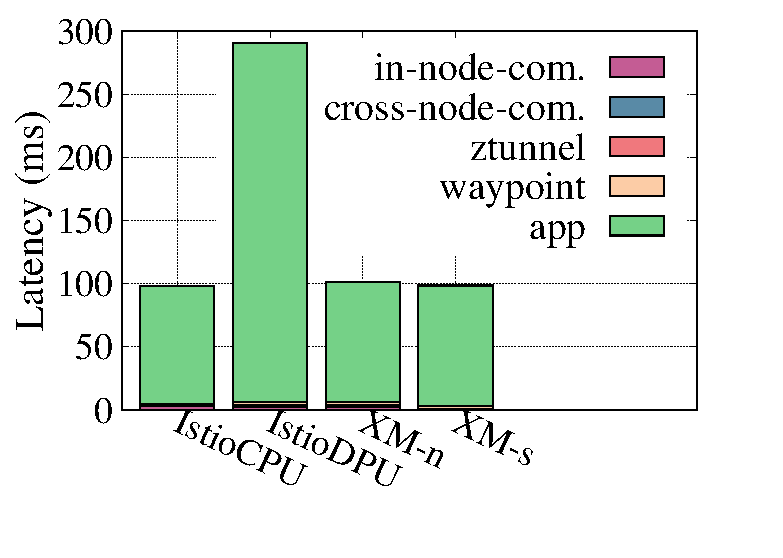
\includegraphics[width=0.99\textwidth]{figs-eval/eval-mesh-breakdown-large.eps}
  \footnotesize \\[-10pt]
  \textbf{(a) Large application.}
  \end{minipage}
\begin{minipage}[t]{0.49\linewidth}
  \centering 
  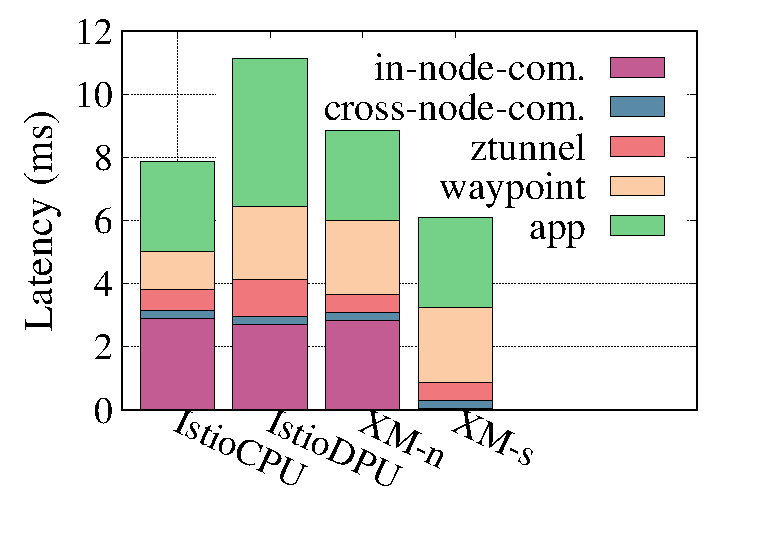
\includegraphics[width=0.99\textwidth]{figs-eval/eval-mesh-breakdown-small.eps}
  \footnotesize \\[-10pt]
  \textbf{(b) Small application.}
  \end{minipage}
 \setlength{\belowcaptionskip}{-15pt}
 \setlength{\abovecaptionskip}{2pt}
  \caption{\textbf{Performance Breakdown (Bluefield2-DPU)}. \textit{XM-n: \sys-Mesh (hetero-netns).} \textit{XM-s: \sys-Mesh (hetero-sock).}}
  \label{fig:eval-mesh-breakdown}
\end{figure}


\myparagraph{Performance breakdown.}
\label{subs:eval-scale}
%We present a breakdown to analyze the improvement from \sys-mesh, using large and small applications.
We present a breakdown using large and small apps.
We break the end-to-end latency into five parts: in-node (including inter-PU and cross-PU) communication latency, cross-node communication latency, and processing latency of ztunnel, waypoint and application.
% We analyze four systems for each application, Istio on CPU (IstioCPU), Istio on DPU (IstioDPU), \mesh using \giptable, \mesh using both \giptable and \gsocket.
As shown in Fig.\ref{fig:eval-mesh-breakdown},
for large app, \mesh (\giptable) can achieve great performance --- 2x better than IstioDPU and almost the same as the IstioCPU performance.
\gsocket brings little improvement here because the processing costs dominate the latency here.
For small app, \mesh (\giptable) outperforms IstioDPU. But it has 16\% higher latency than IstioCPU due to the increased latency on waypoint.
\mesh (+\gsocket) can further improves the latency by optimizing the communication latency, and achieve even better performance compared with IstioCPU.
